%\graphicspath{{images/chap2/}}

\section{Acquiring Organisms}
\epigraph{The following section was written by Lidia Bobrovnikova}{\textit{iGEM LMSU 2021}}
\subsection{Culture Collections}
\subsubsection{Biological collections: purpose and classification}
Biological collections constitute a fundamental heritage of information and knowledge about fauna, flora, and microbiota. They specialise in maintaining and depositing both strains of microorganisms and cell cultures of macroorganisms. Biological cultures are essential in the building of knowledge based on biodiversity. Apart from that, these safe depositaries of biological materials contribute to the acquisition of taxonomic, physiological, genetic, morphological, chemical, and ontogenetic information significantly. 
\newline\newline
Overall, culture collections can be parted into two basic categories: serve collections and work collections. Serve collections possess a great financial support from the government due to their strategic role in development of scientific research and profitability in face of distribution of strains. They are equipped with fully computerised systems of data acquisition and analysis and include large collections of strains and professional curation to serve collections. Work collections often have a comparatively modest number of strains in comparison and have a simpler and non-automated maintenance. They also typically lack robust documentation, collection management, and specialized and efficient delivery service. However, work collections are of a local, regional, and sometimes national importance, fostering various forms of research development and applications of living organisms.
\newline\newline
Ideally, all living biological collections should be affiliated with the World Federation for Culture Collections (\href{http://www.wfcc.info}{WFCC}). Founded in 1963, the WFCC is an entity that collects living biological collections of all natures in the world. About 770 culture collections from 76 countries are currently registered at the WFCC International Data Centre, with varying degrees of organization and activities (research, services, comprehensive collections, professional curation, etc.). Only about 5\% of WFCC-linked collections can be classified as service collections. The WFCC holds periodic events (e.g., the 15th International Culture Collections Conference, held in Chile in November 2019), publishes documents and studies, organizes thematic meetings, and, through organized discussions among its members, establishes actions and defines standard procedures for the operation of biological collections, such as storing strains, distributing control, security procedures, organizing collections, etc. In addition, the WFCC offers a scientific advisory service to help organize malfunctioning collections.

\subsubsection{Microalgae, cyanobacteria and plant tissue culture collections}
Isolation of new strains can be a long and tough procedure. Once isolated they can be maintained without any time limits. However, this is not often the goal for researchers and organising culture collections is a solution in this case. Microalgae and cyanobacteria culture collections are laboratories specially prepared to receive and keep organisms indefinitely, but always presumably in the long term. 
\newline\newline
Culture collections of microalgae are organized mainly according to the existing strains, and secondarily by the microalgae species. This treatment results from counting each culture derived from an isolation event as a unit, regardless of the number of species involved. Thus, very specialized microalgae collections are recognized, with a very small number of species, but with many strains in cultivation. 
\newline\newline 
Overall, collections were divided by \href{https://www.elsevier.com/books/algal-culturing-techniques/andersen/978-0-12-088426-1}{(Lorenz et al., 2005)} into three categories: 
\begin{itemize}
    \item Diverse collections dedicated to research and educational purposes
    \item Collections with well-defined delimitations of species or strains for research or practical study; and
    \item Collections of genetically well-defined and stable strains (often formed by a single
species or a few species) for molecular studies, development of biotechnological applications, etc.
\end{itemize}
\noindent
There are a number of requirements for culture collections. Firstly, all cultures must propagate in aseptic conditions. Secondly, the laboratory must possess enough space for hundreds and thousands of flasks and Petri dishes and supply all the cultures with enough light, CO2, movement of flasks and temperature regimes. Thirdly, for all the strains the appropriate liquid and/or solid medium must be selected.  The lack of the aforementioned factors might cause certain strains to exhibit morphological characteristics different from those typically seen in nature (e.g., reduced size of diatom frustules, pigmentation changes, loss or reduction of cellular projections). And finally, misidentification and accidental mixing of strains should be strictly circumvented and constantly checked. 

\subsubsection{Identification of cultures}
The maintenance of multiple strains in cultures necessarily implies the existence of an adequate identification system of each component of the collection. When few strains exist in a laboratory, controlling the identification of each material is easy and often this aspect is of little importance, as one simply writes the name of the species on the culture flask. In some laboratories, identification is done by an abbreviation of the species name, followed by elements that allow the strain in question to be readily identified. Thus, hypothetically, the cyanobacterium Synechocystis pevalekii could be identified as “SYN PEV.” An isolated strain from Guarapari waters, in Brazil, could be incorporated as SYN PEV GR1, whereas a second strain of the same species isolated from the same place could later be incorporated into the collection as SYN PEV GR2. If a new strain of the same species is isolated in another location, such as Sa\~{o} Lu\'{i}s (also in Brazil), the strain could be classified as SYN PEV SL1. The date on which the culture was inoculated should be indicated on the flask and the use of a diary, in which a continuous record of routine collection maintenance activities is made, may be sufficient to keep the cultures under control. However, the more huge the collection is, the more complex the identification process becomes. 
\newline\newline
One the one hand, it is necessary to characterise a strain from the phylogenetic point of view. This can be conducted by SSU, ITS1, ITS2, 16S/18S and some other constitutive sequences analisis. SSU and 16S/18S data provide researchers with an opportunity to build a phylogenetic tree and see the percent of relatedness of the strain with other organisms. And ITS1 and ITS2 secondary structures enable us to investigate the precise difference of very relative strains. 
\newline\newline
On the other hand, a physiological and biochemical characterisation of strains can also provide us with useful data. Some culture collections not only identify new strains, but also characterise its biotechnological potential. By that growth rate and productivity on different media, a tendency to accumulate certain storage compounds (TAG, starch, etc) or production of any particular molecules is meant. 

\subsubsection{Some culture collections around the world}
Large microalgae collections are part of the reality of some countries, providing an important service to the public. Examples of such centers are the Provasoli-Guillard National Center for Marine Algae and Microbiota (NCMA) (East Boothbay, Maine, USA), Sammlung von Algenkulturen G\"{o}ttingen Universität (SAG) (G\"{o}ttingen, Germany), Culture Collection of Algae and Protozoa (CCAP) (Oban, United Kingdom), and Australian National Algae Culture Collection (ANACC) (Hobart, Australia), Collection of microalgae and cyanobacteria of the Institute of Plant Physiology RAS (IPPAS) (Moscow, Russia), among others. The aforementioned institutions function as units that centralize the national distribution of strains to users for all types of culture uses and applications. These are centers maintained with government resources, but which have the sale of strains as a source to cover (at least partially) the expenses associated with the maintenance of the collections.
\begin{itemize}
    \item \href{http://www.algalresourcescollection.com/}{Algal Resources Collection (ARC)University of North Carolina Wilmington}
\item \href{http://www3.botany.ubc.ca/cccm/}{Canadian Center for the Culture of Microorganisms (CCCM)Vancouver, Canada}
\item \href{http://www.csiro.au/en/Research/Collections/ANACC}{CSIRO Collection of Living Microalgae (CCLM)Australia}
\item \href{http://www.chlamy.org/}{Chlamydomonas Genetics Center (CGC)North Carolina, USA}
\item \href{http://botany.natur.cuni.cz/algo/caup.html}{Culture Collection of Algae at Charles University (CAUP)Prague, Czechoslovakia}
\item \href{http://www.ccac.uni-koeln.de/}{Culture Collection of Algae at the University of Cologne (CCAC)Cologne, Germany}
\item \href{http://algae.ihb.ac.cn/English/}{Freshwater Algae Culture Collection at the Institute of Hydrobiology (FACHB)}
\item \href{http://www.iam.u-tokyo.ac.jp/index.html}{Institute of Applied Microbiology (IAM)Tokyo, Japan}
\item \href{http://www.nbrc.nite.go.jp/e/}{NITE Biological Resource Center (NBRC)Chiba, Japan}
\item \href{https://www.pasteur.fr/en/public-health/crbip/distribution/pcc}{Pasteur Culture Collection of Cyanobacterial Strains (PCC)Paris, France}
\item \href{http://www.uni-goettingen.de/en/184982.htmlhttp://www.uni-goettingen.de/en/184982.html}{Sammlung von Algenkulturen (SAG)Göttingen, Germany}
\item \href{https://www.tistr.or.th/tistrnew/main/index.php}{Thailand Institute of Scientific and Technological Research (TISTR)}
\item \href{http://www.wfcc.info/}{World Federation for Culture Collections (WFCC)}
\item \href{https://www.nies.go.jp/index-e.html}{National Institute for Environmental Studies, Japan}
\item \href{https://utex.org/}{UTEX Culture Collection of Algae at UT-Austin}

\end{itemize}

\subsection{Nagoya Protocol}
\epigraph{The following section was written by the MADRID\_UCM Team}{\textit{iGEM Madrid 2021}}
\subsubsection{What is Nagoya Protocol}

\begin{wrapfigure}{r}{0.3\textwidth}
  \begin{center}
    
\includegraphics [width=50mm] {images/chap1/Working with Phototrophs/Acquiring organisms/image1.jpg}
  \end{center}
 \caption{The Nagoya Protocol was adopted during the 2010 COP10 congress.}
\end{wrapfigure}
\FloatBarrier


The Nagoya Protocol is an international treaty developed by the Convention on Biological Diversity (CBD): the international legal instrument of the United Nations for biodiversity related affairs. It was adopted in 2010, during the 10th conference of the CBD in Nagoya. However it did not enter into force till October 2014. \\ \\
The Nagoya Protocol is an international legally binding protocol on access to genetic resources and benefit-sharing. Its main objective is to define fair and equitable sharing rules for the utilization of genetic resources and their derived benefits, thus contributing to the conservation and sustainable use of biodiversity. \\ \\ 
Thus, the protocol seeks to create a transparent legal framework for access to genetic resources in each region and the fair and equitable participation in the benefits derived from their utilization. Currently the protocol has been signed by more than 150 countries, leading to the creation of specific legal procedures within each one of them for biological resources accession from either national or international entities. \\ \\
Before the Nagoya Protocol, industrialised countries had no legal obligation to ensure fair sharing of the benefits arising from the use of genetic resources. After Nagoya participating countries are obligated to take legal, administrative or policy measures to ensure compliance with legislation governing access to genetic resources and benefit-sharing in the countries providing them. This means that before Nagoya protocol there were no clear procedures that ruled the usage of native biodiversity from a region or requesting access to it. \\ \\
Eventually, the Nagoya Protocol provides a range of recommendations, tools and mechanisms provided to assist contracting Parties. Among these resources there is the recommendation for  establishing national focal points (NFPs) and competent national authorities (CNAs) to serve as contact points for information, grant access or cooperate on issues of compliance.  \\ \\
Other remarked aspects are the creation of an Access and Benefit-sharing Clearing-House to share information, the creation of infrastructure to support key aspects of Nagoya protocol implementation and the financial support for capacity-building and development initiatives through the Nagoya Protocol’s financial mechanism, the Global Environment Facility (GEF). \\ \\
To sum up, Nagoya Protocol aims to raise awareness and promote initiatives for the protection of biodiversity and fair distribution of biological resources. To do so, the protocol establishes an international legal framework that regulates not only the access to biological resources but also the fair distribution of benefits derived for its utilization. Then most of the countries will increase their interest in biodiversity protection and easing the access to its biological resources, due to the potential benefits derived from its utilization either by their own nation or other international entities. 

\subsubsection{Acquiring Novel Organisms Protected Under Nagoya Protocol}
Despite the Nagoya protocol establishes main guidelines and provides recommendations to promote ease the access to genetic resources and benefit-sharing, the final legislations are individually performed by each country, following the recommendation of Nagoya Protocol. \\ \\
After the Nagoya Protocol  entered into force, many countries started protecting their biological resources under the shield of the treaty, especially developing countries looking to secure their regional biodiversity as a potential resource of the country. This way, most of the countries developed a national legal framework to regulate the access to national biological resources and created competent national authorities for biodiversity. \\ \\
For the researcher/institution interested in working with an organism that has been discovered in a region that has decided to regulate the access under the Nagoya framework, this translates into heavy bureaucracy that sometimes can be expensive and highly time consuming. \\ \\
Despite the Nagoya Protocol establish general guidelines to generate a set of terms for a mutual agreement for access and benefit sharing, the complexity of these tramits can widely depend on the country where the organism has been discovered and the intended usage of the organism by the receiver. \\ \\
In general terms, any access request for an specific organism protected by Nagoya protocol consists in the following steps:

\begin{enumerate}
\item First, a formal request has to be submitted to the biodiversity Competent National Authority (CNA). It is common that the submission of this form usually is followed by some type of administrative taxes. This request consists on a document providing personal information as well as information regarding the biological resource access is intended to. Information that is usually required refers to .
\begin{enumerate}
\item Type of biological resource, for example bacteria, plants, soil etc...
\item Amount of resource that is required.
\item Procedure for acquiring the resource for example request to an specific culture collection, field sampling or collection and shipment by a regional collaborator.
\end{enumerate}
\item Secondly, the provided documentation is revised by the CNA. This process can take from some weeks to months. After the revision, the CNA contacts the applicants informing them if they require further clarifications about the requested biological resource and potential derived benefits from its usage by the applicants. 
\item Once the CNA has approved the initial submission, usually they provide the applicants with the official documentation to fulfill. 
It is mainly composed of a document of Mutually Agreed Terms for Benefit Sharing (MAT-BS) which summarizes all the formerly submitted information, as well as a more detailed description of what kind of research or use is going to be performed with the biological resource and which mechanisms are going to be implemented for sharing the potential benefits derived from the usage of the biological resource.
Likewise an Internationally Recognized Certificate of Compliance is usually provided. In this document a the applicant can globally demonstrate their legal compliance with
the nationally established Access and Benefit Sharing (ABS) legislation. Applicant can also define what part of the information provided in the previous documents regarding the usage of the biological resource is confidential and should not be revealed. While the MAT-BS is only accessible to the CBD (Convention for Biological Diversity) and the CNA (Competent National Authority).
\item After fulfilling the provided documentation and its revision by both parts, it must be signed according to the established procedure by the CNA. This final signing procedure usually involves specific tramits that will depend on the country providing the resource. 
\item Once the documentation has been signed by the applicant and submitted to the CNA, a second payment for the administrative taxes can be required. Once this payment is performed and received by the CNA, the responsible  CNA manager signs the documentation and forwards it to the applicant, accompanied by a final approval letter emitted by the CNA.
\item The approval letter is the final document that allows the applicant to access the biological resource. In the case of specific organisms such as cyanobacteria, microalgae or plants maintained in a culture collection, this document must be attached with in addition with the conventional documentation for requesting a strain within the collection.  It is also important to consider that most of the Mutually Agreed Terms documents specify the entity responsible for providing the biological resources to the applicant, forcing them to acquire the organism specifically from that source. 
\end{enumerate}
It is also important to remark that in the MAT-Bs a duration for the usage of the biological resource is established. This duration can be modified or extended depending on the goals of the proposed usage of the biological resource. 


\subsubsection{A real case. Accessing a Novel Cyanobacterium Strain Discovered in India}
\textit{Synechococcus elongatus} PCC11801 is a novel fast growing cyanobacteria discovered in Powai Lake from samples collected in 2015. The iGEM Team MADRID\_UCM 2021 intended to work with this Strain. The experience of this team is going to be explained below, as an example of what a procedure for accessing Nagoya protected strains can look like. 

\begin{formal}
We, MADRID\_UCM 2021 team tried to access PCC11801 directly from the Institute Pasteur. After asking the Institut Pasteur Culture Collection of Cyanobacteria (PCC) they replied that access can only be granted after receiving permission from the National Biodiversity Authority of India (NBA), the CNA of the country.  \\ \\
The process to access the strain followed the formerly described steps, where an initial form was fulfilled online and sent to the NBA. For accession to biological resources from non-Indian parties this corresponds with the Form I that can be found online in the \href{http://nbaindia.org/content/26/59/1/forms.html}{Forms Page} of NBA. Before submitting the form, a payment of 100,000 Indian Rupee is required. This payment can be performed online via a link provided during the submission procedure. (20th of March). \\ \\
After submitting the documentation the revision period started, taking one month to receive a reply from the NBA. In this reply, certain information formerly provided during the online submission was required again as well as additional personal data. After sending all the required information NBA took near 3 weeks to reply the email, requesting some additional clarifications of the provided information. Eventually, two months and a half after the online application, we received an email from NBA, providing us the official MAT-BS and IRCC documents to fulfill and duly sign (27th of May).\\ \\
After fulfilling the documentation and sending back to NBA, the took another couple of weeks to reply. In this moment they asked us for duly signing the documents in every page and sending two copies accompanied by official Indian Stamp paper. In addition a second payment of 5,000 Indian Rupees should be performed. Since Indian Stamp paper is not available in our region and we did not received information regarding how to perform the payment, we wrote an email asking for payment procedure details, as well as alternative options for Indian Stamp paper. \\ \\
The following months consisted on an exchange of several emails where the NBA mainly stated that we still needing to send two duly signed copies in Indian Stamp papers and not mentioning more information regarding the payment of the taxes. Eventually we managed to contact the person responsible for scientific affairs within the Spanish Ambassy in India. Via this diplomatic contact we eventually managed to contact the NBA and send the required documentation via the ambassy to the NBA. We also received the bank account information and payment details via this contact. \\ \\
One week after the payment of the 5,000 Rs tax, NBA sended us the receipt of the bank transfer, asking us for concept of the transfer. We discovered that from the 5,000 Rs that were sent, only 3,555 arrived. We performed a second payment by the value of 2600 Rs, expecting that despite some of the money would be “lost“ during its way, the required amount of 1445 Rs could reach NBA. After two weeks, we received a notification that only 1,248 Rs arrived, and the import of 197 Rs still required to received the approval. After asking our bank and the National Bank of India about possible commissions that we were not advised beforehand and not receiving a clear answer, we eventually found that in any transfer performed to NBA in EUR (€) the import of 15 € was charged to the transfer for currency exchange. Then we performed a final payment of 1,700 Rs and in two weeks we received the confirmation that the money arrived properly accompanied by the signed approval letter. \\ \\
The whole process took around three months, receiving the approval letter the 17th of August from the NBA. Once received we started the request of PCC11801 to the PCC, receiving the strain eventually the 1st of September. 
\end{formal}

\subsubsection{Our Conclusions}

Despite the appealing features of Novel Discovered organisms protected under de Nagoya Protocol, the required legal procedures are long and expensive. This natura make them incompatible with the reduced duration of iGEM Teams experimental research.  If you are planning to work in your (iGEM or not) project with any strain protected under Nagoya Framework, we highly recommend you to first search for similar strains with free access for research or other purposes. If you decide to access a Nagoya Protected Strain, we highly recommend you to start at least 6 months in advance the time you are planning to start working with the strain. \\ \\
Depending on the country where the strain has been discovered the bureaucracy can be more or less agile, however in any case the procedures are more laborious, expensive and time consuming than requesting a strain which is not Nagoya protected. \\ \\
In the particular case of National Biodiversity Authority of India, they usually take around one to two weeks to reply emails. Then, trying to properly prepare all the documentation and performing payments just once can speed up the tramits. \\ \\ 
We have found that any payment performed in EUR to their account in the \textit{State Bank of India} is charged a fee of 15€ by currency exchange. To avoid long waiting times we highly recommend to perform the transfer by other systems like \textit{Xoom} (Paypal Bank Transfers Service), this way the money reaches its destination with the exactly transferred import. 

\subsubsection{Further Reading}
Full Text of Nagoya Protocol Available at CBD page at: \href{https://www.cbd.int/abs/text/}{https://www.cbd.int/abs/text/} \\ \\
F.A.Q About Nagoya Protocol Available at CBD page at: \href{https://www.cbd.int/abs/about/}{https://www.cbd.int/abs/about/}


\section{Growth \& Cultivation}
\epigraph{The following section was written by members from the Bielefeld team}{iGEM Bielefeld-CeBiTec 2021}
\subsection{Higher Plants}
Growing higher plants depends on the options you have in your laboratory and the purpose of the plants. Given the rather undemanding nature of plants there are a lot of different systems in varying complexity. Here we will focus on indoor-methods since those are reproducible and suitable for S1+ plants. Independent of the used methods and materials predetermined standard conditions should be applied.
\newline\newline
The main variables are the medium (in soil, hydroponics or agar or in vitro on plates), the lighting, the temperature and, depending on the used system, the water. Optimal conditions can vary between species. 
\subsubsection{Growing in Soil}
When cultivating in Soil there are a few general things to consider. To prevent compacting of the soil and fungi growth vermiculite, perlite, or polystyrene pellets are mixed with the soil. \\
Before use the soil can be treated with pesticides to prevent plant damage through insects and also fungi growth. Autoclaving the soil is possible but not recommended because this can change the soil properties. The pots for the plants should be sterilized, especially when reused and have drainage holes.
Fertilizer can be added to the soil or the water. For watering distilled and deionised water should be used for reproducibility \parencite{Podar2012}.

\subsubsection{Hydroponics}
For a hydroponic system the seedlings can either be raised in sand that is removed once the roots are long enough or in seedling-plugs which let the roots come out at the bottom. \\
Depending on the aim of the hydroponic system containers, different in size, volume and number of plants per container can be used. The containers should be opaque and have lids to prevent algae growth, evaporation and to create appropriate conditions for root-growth. A light colour can help decrease the temperature of the liquid inside as it may heat up in greenhouses or under certain grow-lamps. \\
When using aluminum for covering, pay caution not to contact the water or to carve the plant: aluminium-salts will form and damage the plant. \\
As holders for the plants, starter plugs made from polyurethane foam, rockwool, or cotton wool can be used. Before planting the seeds the plugs should be soaked in medium to allow pH-adjustment of the plugs.\\
Aeration pumps should be added to the containers to aerate the medium solution. \\
For larger systems instead of containers pipes and a pump system that pumps medium through the pipes are possible. 
Nutrient solutions should consist of distilled and deionised water complemented with nutrients, standard nutrient solutions like \href{http://pmb.berkeley.edu/newpmb/faculty/arnon/Hoagland_Arnon_Solution.pdf}{Hoagland's solution} will work, for different species alterations can be made \parencite{Podar2012}.

\subsubsection{Growing on Plates}
For growing plants on plates, petri dishes and medium are needed. Standard medium is based on  \parencite{Murashige1962} and should be sterilized. The plates can be made like usual plates for bacteria using the plant medium. Once firm, sterilized seeds can be placed on the agar. Horizontal and vertical placing of the plates is possible, vertical placing allowing better root development \parencite{Podar2012}. 

\subsubsection{Lighting}
The other big factor in plant growing besides nutrition is the lighting. First of all a light source is needed. Maybe the greenhouse of your university can supply you with lamps or you can grow your plants directly in it, otherwise there are numerous growth shops (mainly national, in Germany and Austria e.g. \href{https://www.grow-shop24.de/}{https://www.grow-shop24.de/} ) that sell grow lamps. LED-lamps, being more efficient and burning cooler, are generally better than conventional light bulbs \parencite{Goto2012}. Depending on the size, number and age of your plants a different lighting system  might be optimal. If you have numerous plants you need a wide covering to make sure every plant gets enough light. This can be verified using a Mini-PAM to measure the fluorescence of the photosystem II in the chloroplast. \\
There are optimal lamps for young plants, for maximal growth and for flowering. The exposure time can also vary and have different influences.

\subsubsection{Temperature}
Obviously plants can grow and survive a broad range of temperatures but if optimal growth is desired and there is the possibility to regulate the temperature of the plants environment it should be done, considering every plant has an optimal growth temperature. For most applications room temperature will be fine though. \\ \\
Below you can find a collection of optimal growth conditions, nutrition etc. for different lab relevant species.

\paragraph{Arabidopsis} \mbox{}  \\
\textit{Light intensity}. Approximate 100–200 μmol/m2 s from fluorescent bulbs, although lower light intensities have also been used (e.g., 40–60 μmol/m2 s \parencite{Podar2012}). Also, higher light intensities of 250  μmol/m2 s provided by mercury vapor lamps have been reported \parencite{Arrivault2006}. \\ \\
\textit{Photoperiod}. Long days >12 h accelerate the reproductive cycle—plants grown under long day regimes produce a small biomass (few and small leaves) while development of inflorescences occurs early. One example is 16/8 h day/night regime at 23/18°C.\\ \\
Short days <12 h favor vegetative growth—a 10 h/14 h day/night regime provides a good compromise between sufficient shoot biomass production and pre-flowering growth \parencite{Gibeaut1997}. \\ \\
\textit{Temperature}. 20–22°C day/17–18°C night. The temperatures required for Arabidopsis growth depends on the ecotype. In general, temperatures around 20–22°C during the day and 17–18°C during the night are fine for any of the ecotypes. However, A. thaliana Landsberg erecta grows better at day temperature around 23°C, whereas Columbia 0 (Col 0) shows stress symptoms at this temperature \parencite{Gibeaut1997}. \\ \\
\textit{Stratification of seeds}. Arabidopsis seeds, depending on the ecotype, can germinate without stratification. However, stratification of seeds ensures a more uniform germination and therefore a better comparison of results between different lots of seeds that are used in an experiment. Stratification of seeds is performed at 4°C for 2–4 days depending on the ecotype. Three days stratification periods would suit any of the Arabidopsis ecotypes. Stratification can be performed before sowing by placing the seeds into a vial in water or after sowing by placing the plates (in vitro experiments) or the pots with soil at 4°C. Seeds can be kept at 4°C for up to a week.\\ \\
\textit{Humidity}. High humidity is required for Arabidopsis seeds to grow, e.g., 65\% \parencite{Peiter2007}, 75 \% \parencite{Gibeaut1997}, 60/75 \% day/night \parencite{Arrivault2006}. \\ \\
Soil. In general, any standard peat-based soil/compost would work for Arabidopsis. Here are two examples: GS90 (composition: peat, clay, coconut fiber, 2 g/L salt, 160 mg/L N, 190 mg/L P2O5, 230 mg/L K2O, pH 6; supplied by Werner Tantau GmbH \& Co. KG, Germany) \parencite{Koslowsky2008} and Levington F2 seed and modular compost pH 6 (Green-tech, UK). Soil is mixed 1:1 v/v with vermiculite or perlite. \\ \\
\textit{Trays/pots}. The size of trays/pots used for Arabidopsis growth depends on the number of plants that are needed for the experiment and available space for growing. In general, people use flat cell trays if individual plants are required or large trays if plants are to be pooled. For trays with individual cells or pots a square of around 7 × 7 cm works well. However smaller cells/pots (36 cells trays) also give good results. \\ \\
\textit{Containers for hydroponics}. One example would be to use a 5 L container 35  ×  35  ×  20 cm, holding up to 36 plants, with a diameter of the hole of 1.5–2.0 cm and a distance between the holes of 4–5 cm.

\paragraph{Barley}\mbox{}  \\
\textit{Light intensity}. Barley requires high light intensities and therefore the light quality can significantly influence the performance of the plants. 350–500 μmol/m2 s photosynthetically active radiation \parencite{Gries1995}, \parencite{Holme2006} is adequate.\\ \\
\textit{Photoperiod}. 16/8 h light/dark photoperiod is used most of the time for barley. \\ \\
\textit{Temperature} The regime varies between experiments and may also depend on whether the conditions in the greenhouse or growth chamber can be adapted for barley or whether other plant species are to be grown. However, keeping the temperature in the low range 10–20°C would be beneficial. High temperatures should be avoided. If plants are to be grown for the whole life cycle then $\sim$15°C/10°C day/night temperatures gives good results \parencite{Holme2006}. Other day/night temperature regimes that can be used are: 20/15°C, 20/17°C, 21/18°C, 23/17°C \parencite{Gries1995} or 24/18°C. \\ \\
\textit{Humidity}. Relative air-humidity varies between different published data, but in general is between 60 and 80 \%. \\ \\
\textit{Soil type}. There are different types of soil that can be used to grow barley, but here are three possibilities that all work well: (1) Standard sphagnum (or sphagnum mixed with polystyrene pellets in a 2:1 ratio), (2) Levington F2 seed and modular compost pH 6 (Green-tech, UK) mixed with perlite in a 3:1 ratio or (3) compost and perlite in a 4:1 ratio \parencite{Murray2004}. \\ \\
\textit{Pots size}. A 2 L pot works well. However, smaller pots (15  ×  15  ×  15 or 13  ×  13  ×  13 cm square) can also be used, but if there are no space constraints, then larger pots would work better. \\ \\
\textit{Containers for hydroponics}. The volume of the containers varies largely between experiments. In general, if the plants are to be grown in hydroponic solution up to maturity and seeds are required 1 L hydroponic solution/ plant is recommended. Alternatively smaller containers can be use such as 5 L containers that can hold up to ten plants. Diameters of the holes should be 2.0 cm and a distance between the holes of at least 5 cm \parencite{Podar2012}.

\paragraph{Rice}\mbox{}  \\
\textit{Light intensity}. Rice, like barley, requires high light intensities and therefore the light quality can significantly influence the performance of the plants. 300–500 μmol/m2 s photosynthetically active radiation \parencite{Miyamoto2001}, \parencite{MartinezAtienza2006}. \\ \\
\textit{Photoperiod}.16/8 h light/dark photoperiod is used most of the time for rice. However 12/12 h  day/night regime can also be used. \\ \\
\textit{Temperature} The regime varies between experiments. However, rice prefers higher temperatures, in general above 20°C. Some examples of day/night temperatures used are: 25/20°C \parencite{MartinezAtienza2006} or 27/22°C \parencite{Miyamoto2001}.\\ \\
\textit{Humidity}. Relative air-humidity varies between different published data, but in general is between 40 and 80 \%. \\ \\
\textit{Soil type}. There are different types of soils that can be used to grow rice; in general clay loam mineral soil should be avoided. Levington F2 seed and modular compost pH 6 (Green-tech, UK) mixed with vermiculite or perlite in a 1:1 v/v ratio works well for rice. \\ \\
\textit{Pots size}. See barley (Subheading 4.1.2). \\ \\
\textit{Containers for hydroponics}. The volume of the containers varies largely between experiments. In general, 0.4–1 L hydroponic solution/ plant is recommended (e.g., 20–24 plants/8–10 L container \parencite{Miyamoto2001} \parencite{MartinezAtienza2006}). Alternatively smaller containers can be use such as 3 L containers that can hold up to 16 plants. Diameter of the hole is 2.0 cm and a distance between the holes of at least 5 cm should be used \parencite{Podar2012}.

\epigraph{The following section was written by members of the Linköping team}{\textit{iGEM Linkoping\_Sweden 2021}}
\subsection{Cyanobacteria}
Growth of Cyanobacteria in Different Conditions
One of the disadvantages of using Cyanobacteria in research is their relatively slow growth rate with a doubling time of 3 hours. The following experiments were therefore performed on the cyanobacteria strain synechocystis sp PCC 6803 to establish optimal growth conditions. \\ \\
For evaluation of growth the optical density was measured every 24 hours at a wavelength of 544 nm. Day 0 started with a base OD of around 0.05 - 0.08, growth was evaluated respectively. \\ \\
The standard medium used for Cyanobacteria is the BG11 medium, the protocol on page (BG11 medium page) was followed. For a real life comparison the groups with autoclaved Brackish and Sea water were added, the samples were collected at the Baltic Sea Island Gotland or the west coast of Sweden near Gothenburg. 

\begin{table}[!htpb]
\centering
\caption{Different Conditions of the growth curve experiment}
\begin{tabular}{|l|l|} 
\hline
\textbf{Name} & \textbf{What is it?}       \\ 
\hline
BG11          & BG11                      \\
pH6           & BG11 at pH 6              \\
pH7           & BG11 at pH 7              \\
pH8           & BG11 at pH 8              \\
Brackish      & BG11 + 3.5\% NaCl         \\
Sea Water     & BG11 + 3.5\% NaCl         \\
Gotland       & Brakish Water autoclaved  \\
Göteborg      & Sea Water autoclaved      \\
\hline
\end{tabular}
\end{table}
\FloatBarrier

\begin{figure}[!htbp]
    \centering
    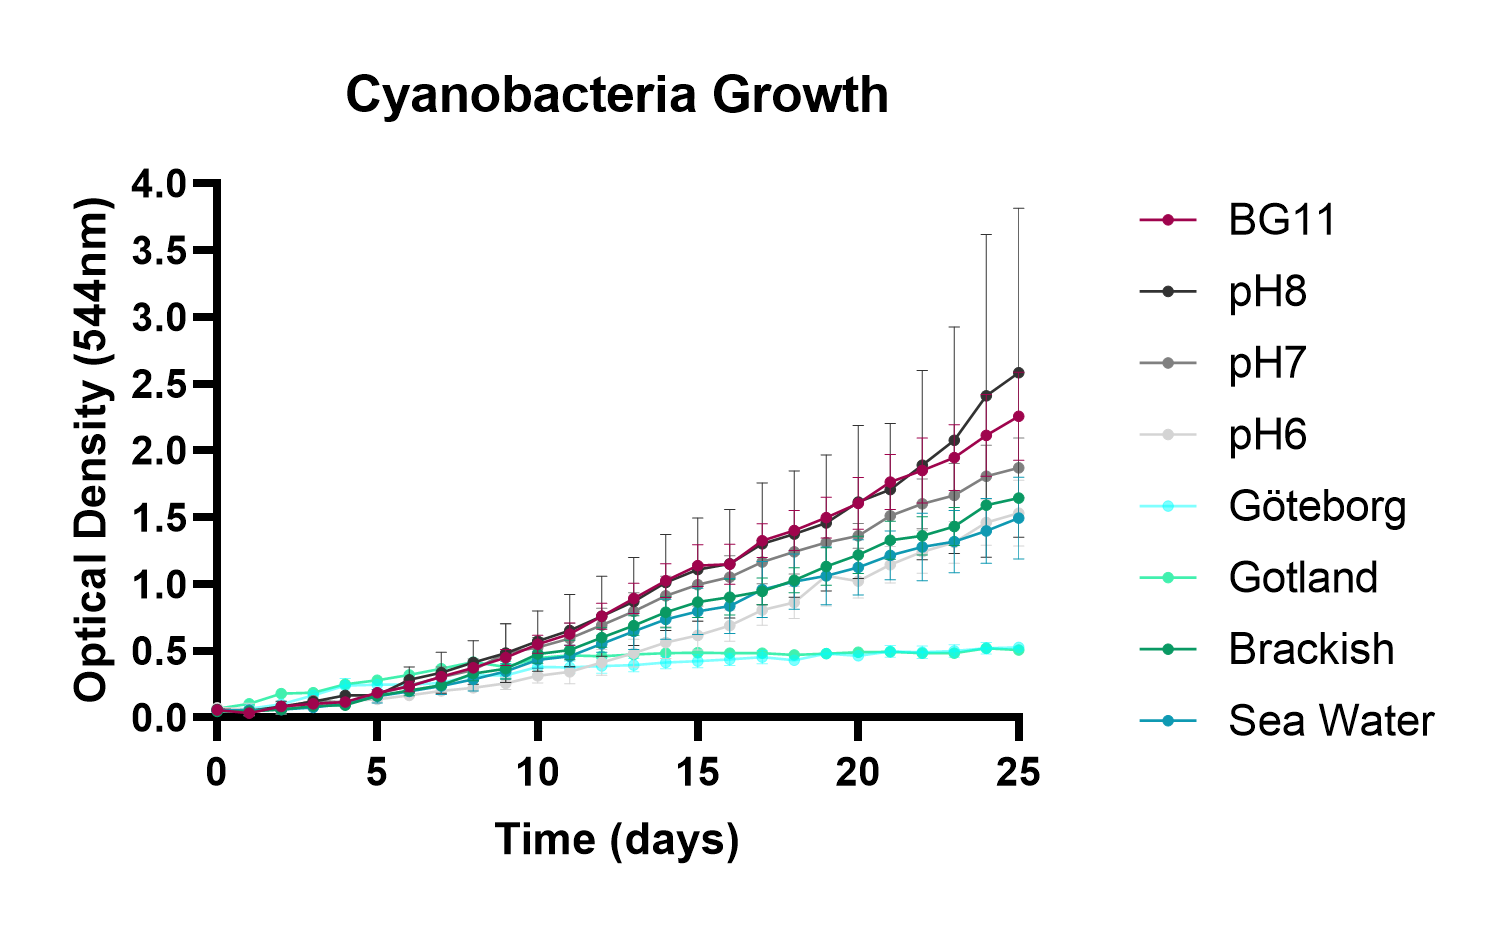
\includegraphics[width=\textwidth]{images/chap2/chap2_cyano_03.png}
    \label{fig:ch2cyano01}
    \caption{Growth curve of synechocystis in different conditions. Optical density at a wavelength of 544 nm was measured every 24 hours. Conditions are as followed: BG11 (standard medium), BG11 with different pHs (6,7,8), BG11 with different salt conditions (Brackish (1.5\% NaCl), Sea Water (3.0\% NaCl)) and water collected from the Baltic Sea and the West Coast of Sweden (Gotland, Göteborg (Gothenburg)). Error bars represent the mean +- SEM from 3 biological replicates. All growth media were autoclaved before the bacteria was added.} 
\end{figure}
\FloatBarrier
\noindent

\subsubsection{Incubator setup and lighting}
Finding standardised lighting and incubator configurations is a difficult task, but acquired data shows that with even simple setups, good growth conditions can be achieved. Normal incubators can easily be turned into incubators suitable for the growth and cultivation of cyanobacteria. In figure 2.3 below, 2 LED lamps emitting 340 lm each were installed with double sided tape in a normal incubator. This generated a light intensity gradient in the incubator, which can be seen below in table \ref{tab:gradients}. Due to the cyanobacteria growing well independently on wherever it was placed in the incubator, the conclusion can be made that the gradient had little effect on the growth condition as a whole. 

\begin{table}[!htpb]
\caption{The different gradients acquired in the incubator after the installation of the lighting}
\label{tab:gradients}
\centering
\begin{tabular}{|l|l|l|} 
\hline
\multicolumn{3}{|c|}{\textbf{Top Level }}       \\ 
\hline
Left~    & Middle   & Right                     \\ 
\hline
5700 lux & 2300 lux & 1300 lux                  \\ 
\hline
\multicolumn{3}{|c|}{\textbf{Bottom Level }}    \\ 
\hline
Left     & Middle   & Right                     \\ 
\hline
300 lux  & 300 lux  & 4000 lux                  \\
\hline
\end{tabular}
\end{table}
\FloatBarrier

\begin{figure}[!htbp]
    \centering
    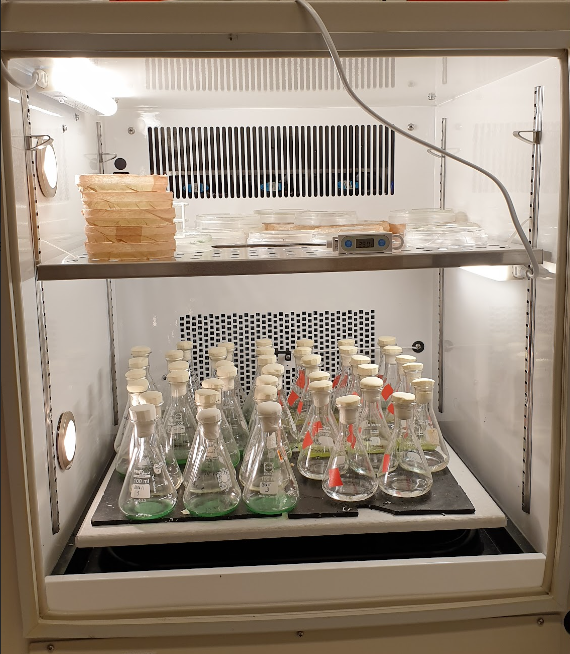
\includegraphics[width=0.7\textwidth]{images/chap2/chap2_cyano_02.png}
    \label{fig:ch2cyano02}
    \caption{Growth curve of Cyanobacteria in different conditions. Optical density at a wavelength of 544 nm was measured every 24 hours. Conditions are as followed BG11 (standard medium), BG11 with different pHs (6,7,8), BG11 with different salt conditions (Brackish, Sea Water) and water collected from the Baltic Sea and the West Coast of Sweden (Gotland, Göteborg). Data is presented ± SEM} 
\end{figure}
\FloatBarrier

\epigraph{The following section was written by members of the Sorbonne team}{\textit{iGEM Sorbonne\_U\_Paris 2021}}
\subsection{Algae}
The "algae" are a polyphyletic group of eukaryotic organisms capable of photosynthesis. Until very recently, the classification of algae was based only on morphological criteria, so that these organisms can be found in many groups of protists, such as Euglenozoa, Stramenopiles or Dinoflagellates. As a result, this group has an incredible phenotypic and genetic diversity, which can be a challenge for their culture as well as an advantage for their isolation. We will focus here on unicellular algae, on which most of the synthetic biology work is currently concentrated, and we will discuss culture and isolation methods for both environmental organisms and reference strains available in the laboratory.
\begin{figure}[!htbp]
    \centering
    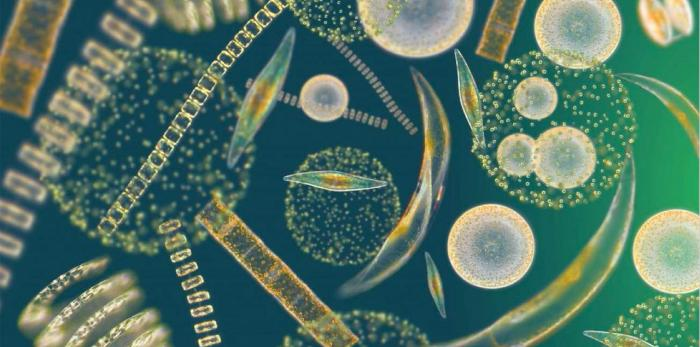
\includegraphics[width=\textwidth]{images/chap2/chap2_alg_01.png}
    \label{fig:ch2alg01}
    \caption{Marine and lacustrine algae do not constitute a homogeneous monophyletic group: as a result, they possess an incredible diversity of forms and functions.} 
\end{figure}
\FloatBarrier
 \noindent
\subsubsection{Isolation of microalgae}
Following a sampling in the field, it may be necessary to concentrate the algae if they are in dispersed or planktonic form. This concentration step can be done by membrane filtration or by gentle centrifugation. The algae can then be quickly identified with an upright microscope before proceeding to their isolation. Several isolation methods exist, and the choice between them depends on the qualities of the targeted algae. All these methods aim at obtaining monoclonal lines.
\paragraph{Direct isolation}\mbox{}\\
Motile algae can be inseminated on an agar medium (0.5\%) with one end hidden from the light. The motile algae will then tend to move towards the light source by phototactism. The algae can thus be isolated directly under an inverted microscope using a tapered Pasteur pipette before being transferred to sterile medium. An alternative is to use an atomizer which sprays water droplets containing isolated algae on the culture medium. Once the colonies are formed, it is then possible to transfer them on sterile medium.
\paragraph{Selective enrichment}\mbox{}\\
Selective enrichment consists in growing the algae in a medium that only allows the growth of certain target organisms and that causes the death or the stop of the growth of undesirable organisms. It is then necessary to adapt the culture media according to the qualities of the alga that we want to isolate. This method therefore requires prior knowledge of the strain that we seek to isolate. Isolation is probably done under an inverted microscope using a tapered pipette \parencite{Richmond2013}.
\paragraph{Streak method}\mbox{}\\
The streak method involves raking the culture solution onto a fairly solid petri dish (about 1\%) and then harvesting the colonies and seeding them within 96-well plates. The grown colonies can then be successively transferred to 48 and 24 wells plates before being put in flasks.
\paragraph{Density gradient centrifugation}\mbox{}\\
The use of a centrifugation gradient to separate algal species of different densities has been performed \parencite{Whitelam1983}using colloidal silica (otherwise called silica sol or Percol). This isolation allows the formation of discrete bands of algae of different density within the Persol gradient.
\paragraph{Flow cytometry and cell sorting}\mbox{}\\
Flow cytometry can also separate microalgae according to their size and pigment content. However, this method can be inaccurate and does not guarantee to obtain an axenic culture \parencite{Richmond2013}.
\subsubsection{Choice between axenic and non-axenic culture methods}
Sometimes the design of a genetic system requires the use of axenic strains. It is then necessary to eliminate all the organisms present in the coculture, whether they are protozoa, bacteria or viruses. Successive transfers on sterile medium as previously described generally allow to obtain monoclonal lines, but do not guarantee to obtain axenic lines. Several techniques can be used to obtain axenic lines. Among these, it is possible to irradiate algal cultures with UV light. Algae are generally quite resistant to UV radiation due to their production of pigments and other metabolites such as mycosporin analog amino acids \parencite{Carreto2011}. However, some bacteria are excellent extremophiles, and it is therefore important to check for the absence of opportunistic bacterial development in environments thus free of predators. Moreover, too much radiation can alter the photochemistry of the alga or induce damage to the algal genome or proteome. Therefore, antibiotics and antifungals are often used to eliminate any bacteria or fungi associated with algal cultures \parencite{Richmond2013}. However, it is observed that after several transfers to sterile media, the cultures tend to become axenic. The relevance of such axenic cultures in synthetic biology is however increasingly questioned. Indeed, several studies have shown that algae often have a set of associated bacteria in the natural environment, equivalent to the human microbiota known as the "cyanosphere". These symbiotic associations can range from the simple exchange of nutrients to the sharing of vitamins, siderophores and even antibiotics. Some articles indicate that bacterial symbionts of \textit{Chlamydomonas reinhardtii} such as \textit{Leisfonia sp.} would increase biohydrogen production by the alga or that different species of pseudomonas associated with Chlorella vulgaris would allow for more biodiesel production \parencite{Yao2018}. The study of symbionts in "domesticated" algae could therefore be crucial in large-scale production perspectives or in the simple maintenance of algal cultures over time. Some algal libraries, such as that of the Muséum National d'Histoire Naturelle in Paris, have already opted for non-axenic cultures, which are less demanding and more sustainable over time.

\begin{figure}[!htbp]
    \centering
    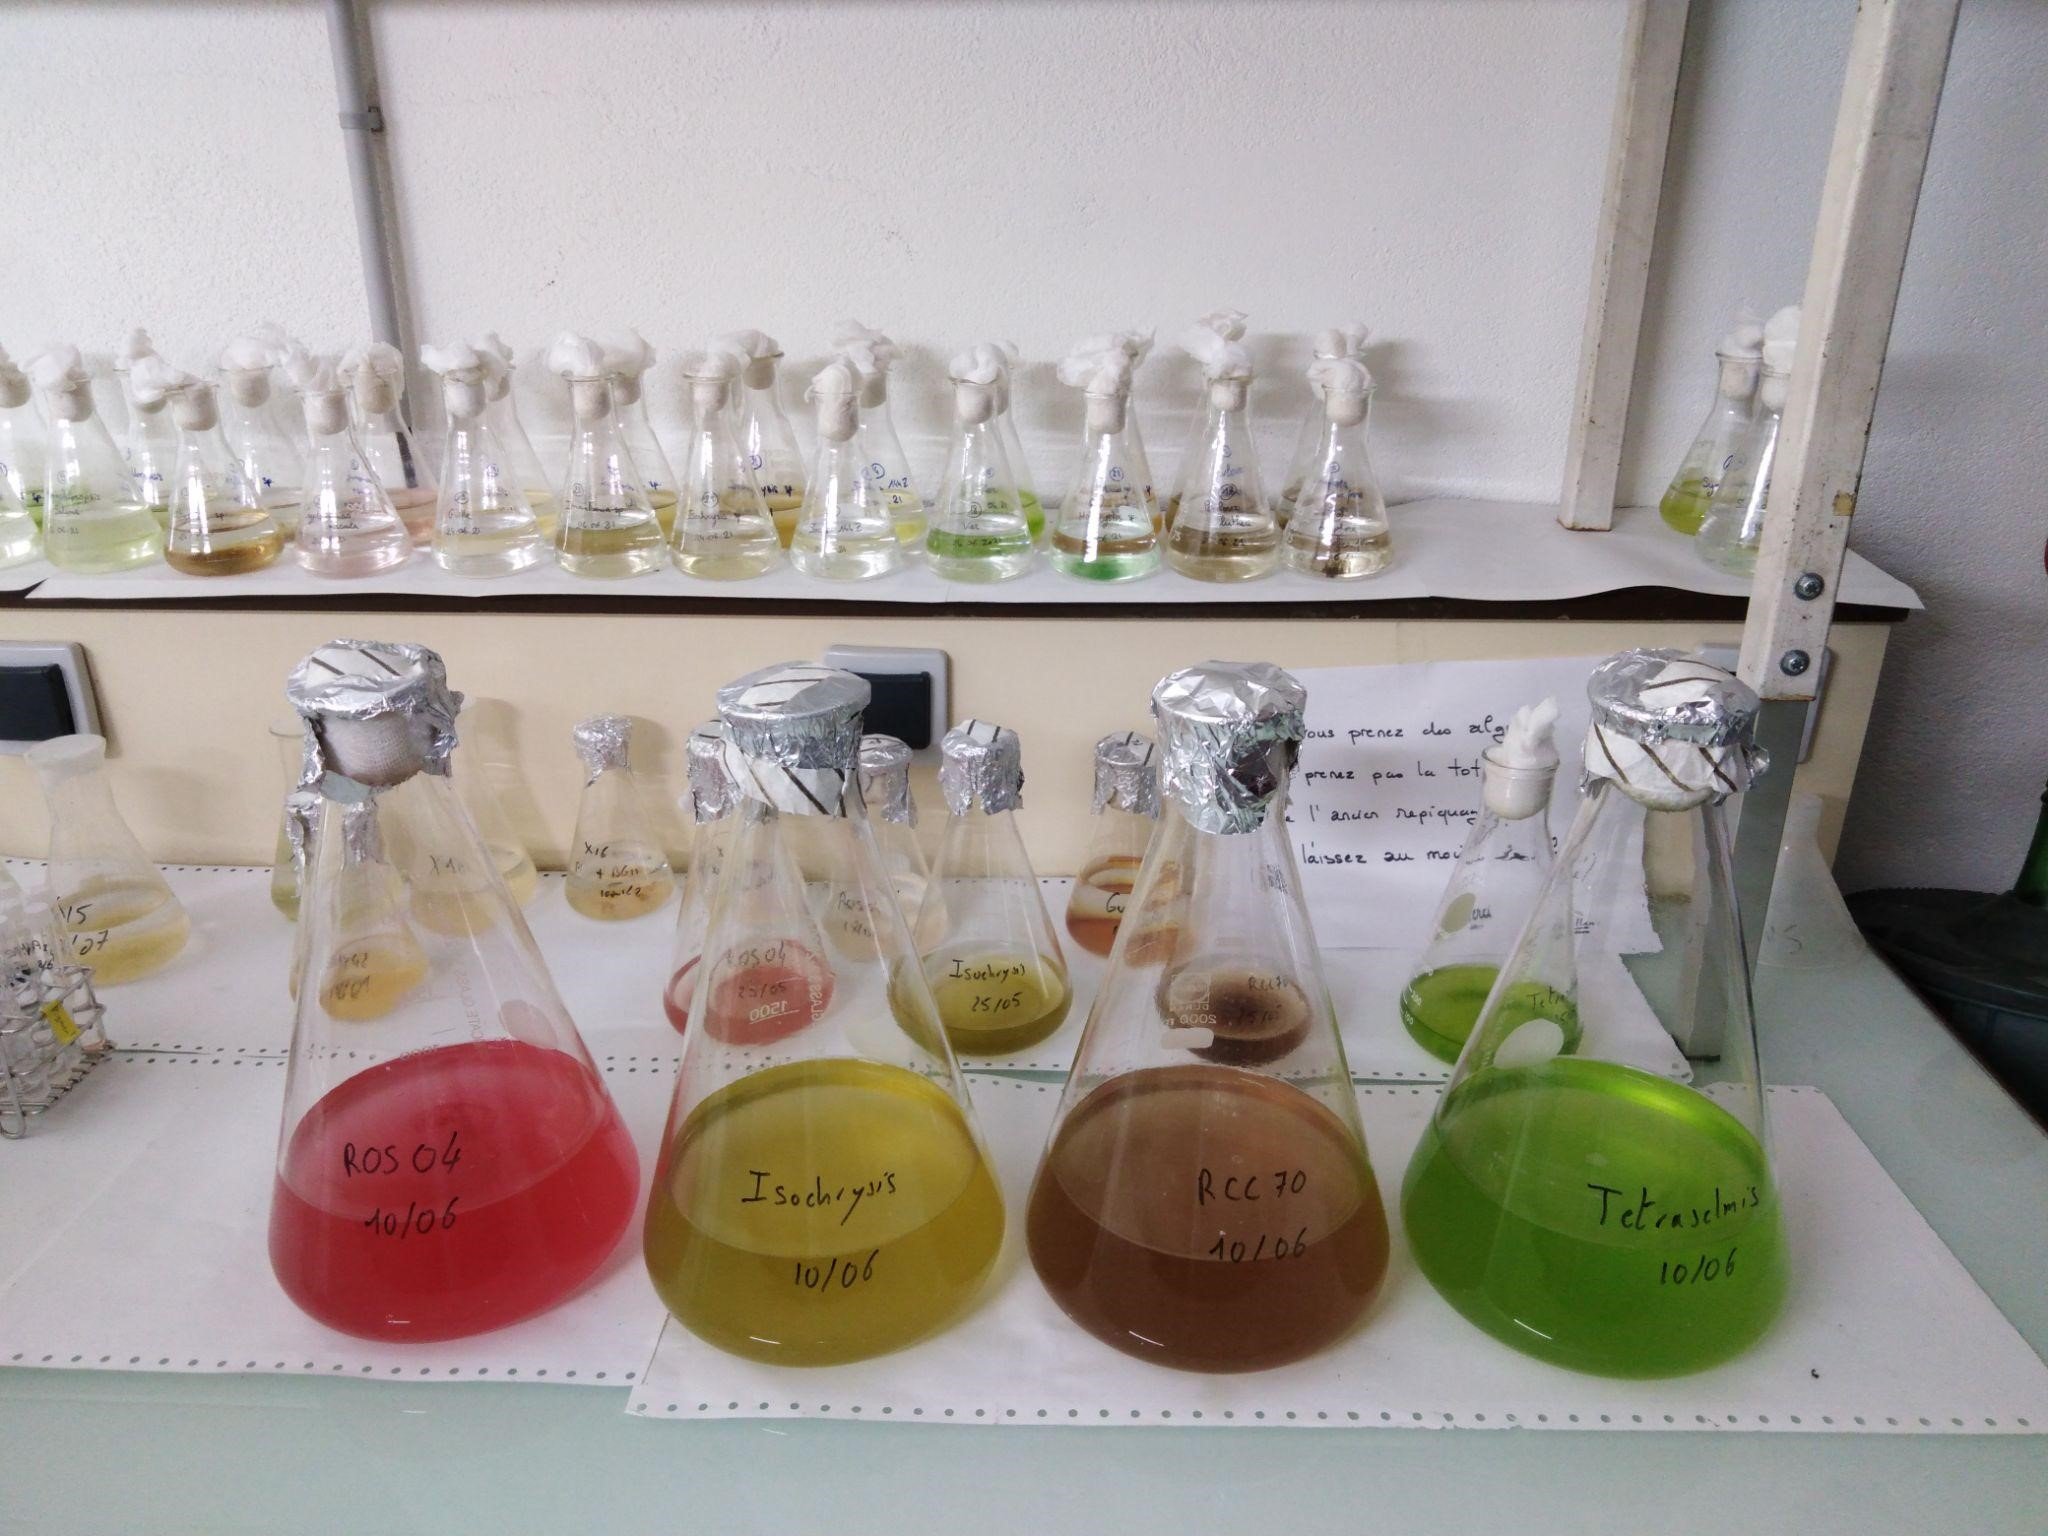
\includegraphics[width=\textwidth]{images/chap2/chap2_alg_02.jpg}
    \caption{Several algal libraries, such as the one at the marine ecology station of Banyuls-sur-Mer (Sorbonne University, France), have adopted a non-axenic culture method that is closer to the conditions of culture in natural environments.}
    \label{fig:ch2alg02}
\end{figure}
\noindent
\subsubsection{Maintenance of algal cultures for strain conservation}
Once the monoclonal cultures are obtained, it is possible to place them in flasks with a cap allowing gas exchanges. The cultures can then be placed in incubators, where the humidity, light and temperature are regulated according to the algae and the desired objective: multiplication of the algae or simple maintenance in the culture medium. For cultures with a large number of different algae, mainly from temperate or warm regions, it is possible to set at 25°C \parencite{Georgianna2012}. Transplanting will then need to be scheduled on a regular basis (usually every two months but to be estimated based on the growth of the algae). Species from temperate regions can be placed at lower temperatures (between 18 and 19°C) to reduce transplanting time, but a higher temperature will still be required for strains from tropical regions. White light lamps or natural light should be favored, in order to give the algae the widest possible spectrum and to have a larger collection, but it is still possible to select certain wavelengths to favor the growth of certain organisms, following research in the literature to verify the absorption spectra of the pigments. The new LED lights have the advantage of being easily positionable and adjustable to the needs of the algae, but a natural light can bring environmental variations whose benefit over time is not to be neglected. Thus, some laboratory scientists report empirically that unchanging environmental conditions (composition of the medium, temperature...) tend to weaken the algal cultures of collections over time, although optimal conditions are favored for mass production, so that experimenters tend more and more to reproduce the natural environment of algae. For simple conservation, the algae can be stored without any agitation in the culture chamber or incubator, but for mass production as often desired in molecular biology, regular agitation on an orbital shaker tray is preferred.
\subsubsection{Main culture media for model organisms in synthetic biology}
In this section, we will mention the main culture media for model algal organisms in synthetic biology.  It should be noted that depending on the metabolic activity targeted during the experiments, it is sometimes necessary to adapt the culture conditions of each alga.
- \textit{Chlamydomonas reinhardtii}: This is one of the algae for which a MoClo Toolkit has been defined \parencite{Crozet2018}, and is therefore one of the most widely used algae in synthetic biology. \textit{Chlamydomonas reinhardtii} has the advantage of being a mixotrophic alga, so it can be grown in heterotrophic media to accelerate yields. The TAP medium (TRIS acetate phosphate) remains the reference medium for the different strains, but the presence of acetate tends to decrease the photosynthetic activity of the alga, it is recommended to use a minimum medium if this activity is part of the parameters to be tested during the experiment. Thus, the HSM medium is used as reference medium for the study of autotrophy in \textit{Chlamydomonas reinhardtii}. Several authors recommend to supplement the TAP medium with different compounds such as phytohormones or antibiotics.

\begin{figure}[!htbp]
\floatbox[{\capbeside\thisfloatsetup{capbesideposition={left,top},capbesidewidth=6cm}}]{figure}[\FBwidth]
{\caption{Cultures of Chlamydomonas reinhardtii. It is possible to monitor the growth of the algae in a very visual way: the greener the culture appears the more concentrated the algae is. Thus, the first Erlenmeyer flask on the left does not contain a sufficient concentration of algae to proceed to a transformation, while those on the right seem to be sufficiently concentrated. More opaque green cultures are usually too concentrated and should be diluted. The medium should appear homogeneous under agitation, otherwise the culture may be contaminated.}
\label{fig:ch2alg03}}
{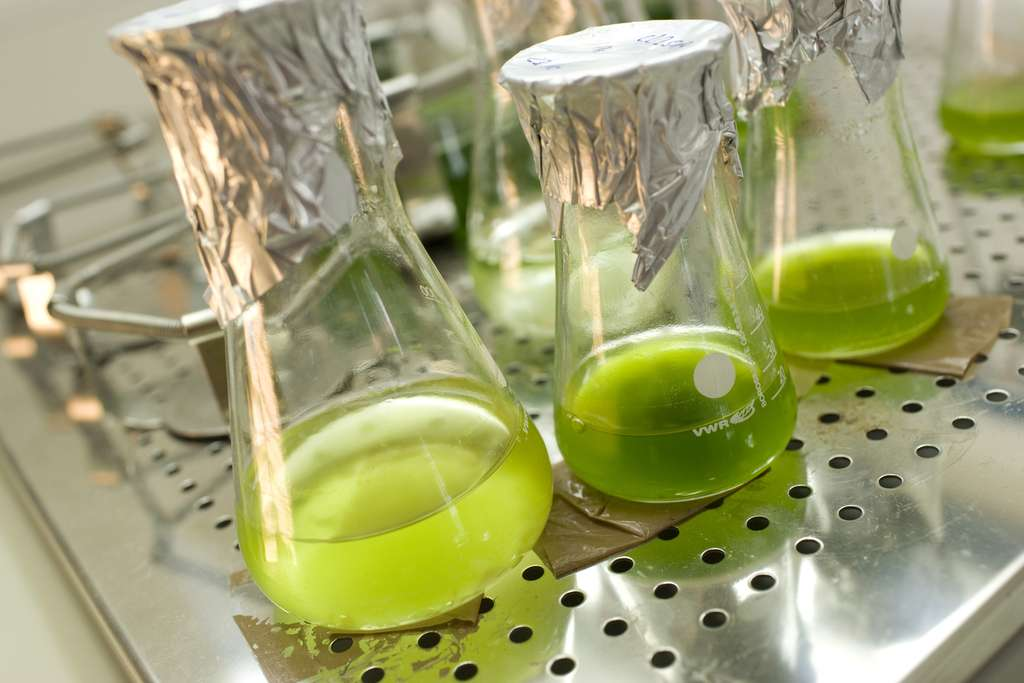
\includegraphics[width=8cm]{images/chap2/chap2_alg_03.png}}
\end{figure}
\FloatBarrier
\noindent
\paragraph{Other informations about the culture of \textit{Chlamydomonas reinhardtii}} \mbox{}\\
The generation time of the cells is 8 hours and the exponential phase is 1 to 5 million cells per mL. Care should be taken to ensure that the cell concentration remains stable during the experiment. The cells are agitated during the whole culture.
Protocol TAP medium: \href{https://www.protocols.io/view/TRIS-acetate-phosphate-TAP-medium-e95bh86}{www.protocols.io}.
Protocol HSM medium : \href{https://www.protocols.io/view/Sueoka-s-High-Salt-Medium-fdebi3e}{www.protocols.io}

\begin{description}
\item[\textit{Ostreococcus tauri}]\mbox{}\\ 
Ostreococcus tauri is the smallest eukaryotic photosynthetic organism known at present \parencite{Chretiennot-Dinet1995}. It is a marine microalga discovered in the 1990s in the Etang de Thau, in the French Eastern Pyrenees. The genome of O. tauri is very short, about 12,513 bp \parencite{Derelle2006}, and has sometimes been cited for synthetic biology studies, mostly for basic research purposes. The algae are grown in ASW (Artificial Sea Water, see composition at \href{https://www-cyanosite.bio.purdue.edu/media/table/asw.html}{www-cyanosite.bio.purdue.edu}) medium within an incubator under a light intensity of about 20 µmol.m-2.s-1 placed at 20°C \parencite{vanOoijen2012}. The cells do not have to be agitated during culture, but the handler must ensure that the algae are resuspended daily.
 
\item[\textit{Phaeodactylum tricornutum}]\mbox{}\\
The diatom \textit{Phaeodactylum tricornutum} represents one of the main hopes of synthetic biology since TALEN endonucleases and the Cas9 system were used to modify its genome \parencite{Kroth2018}. \textit{Phaeodactylum} cultures are placed under agitation (120 rpm), at a temperature of 22°C and an irradiance of 152 µEinstein.m-2.s-1. The composition of the algal culture medium is given within the article by \parencite{Bitaub2008} available at \href{https://www.sciencedirect.com/science/article/pii/S1369703X08000648}{https://www.sciencedirect.com/science/article/pii/S1369703X08000648}
 
\item[\textit{Thalassiosira pseudonana}] \mbox{}\\
This is another model diatom in synthetic biology for which the Golden Gate cloning method is applicable, but for which there is not yet a MoClo toolkit \parencite{Kroth2018}. Cells are placed at 20°C with agitation in ASW medium (see \textit{Ostrococcus tauri}) supplemented with 1 µg.L-1 vitamin B12 \parencite{Cook2015}.
 
 \begin{figure}[!htbp]
\floatbox[{\capbeside\thisfloatsetup{capbesideposition={right,top},capbesidewidth=6cm}}]{figure}[\FBwidth]
{\caption{The diatom \textit{Thalassiosira pseudonana} (above with its two silica frustules) represents one of the main hopes of synthetic biology, although no MoClo toolkit has yet been created for it.}
\label{fig:ch2alg04}}
{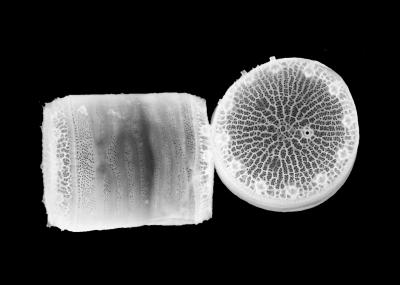
\includegraphics[width=8cm]{images/chap2/chap2_alg_04.png}}
\end{figure}
\FloatBarrier
 \noindent
\item[\textit{Dunaliella salina}] \mbox{}\\ 
Dunaliella is known to be one of the major commercial sources of β-carotene, but its significant production of lipids, proteins, and vitamins makes it likely to become a synthetic biology model in its own right in the future. The pigment color of the cell depends on the salinity of its environment: Dunaliella turns red when exposed to salinities above 25\% because it then loads up with carotenoids. Dunaliella salina is only autotrophic, the quality of the light to which it is exposed is thus very important, this light must be natural or white. Its optimum temperature is between 25 and 35°C and its optimum pH between 9 and 11. This alga requires a continuous supply of CO2, either in the form of gas or 10 mmol.L-1 of NaHCO3 \parencite{Hosseini2009}. The optimal culture medium for obtaining β-carotene is described in the article by \parencite{Morowvat2016} available at \href{https://www.sciencedirect.com/science/article/pii/S1878818116301773?via\%3Dihub}{https://www.sciencedirect.com/science/article/pii/S1878818116301773?via\%3Dihub}.

 \begin{figure}[!htbp]
\floatbox[{\capbeside\thisfloatsetup{capbesideposition={left,top},capbesidewidth=6cm}}]{figure}[\FBwidth]
{\caption{\textit{Dunaliella salina} changes color according to the salinity of the environment}
\label{fig:ch2alg05}}
{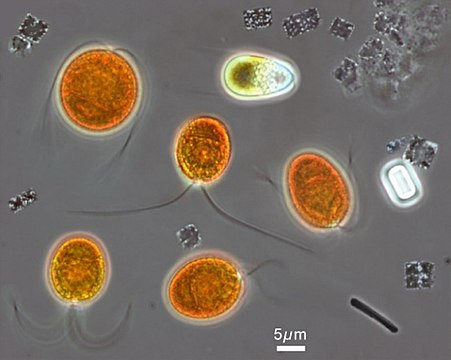
\includegraphics[width=8cm]{images/chap2/chap2_alg_05.png}}
\end{figure}
\FloatBarrier
\end{description}